\documentclass{jsarticle}
\usepackage[dvipdfmx]{graphicx}
\begin{document}

\title{身体動作と筋電量の関係性}
\author{平松亨隆}
\maketitle


\section{目的}
私を含めて人は、体を動かすときに意識的に筋肉の伸縮を考えて体を動かすわけではない。だから、我々は体を動かすときに筋肉が具体的にどのように働いているかを知らない。そこで、調べてみることにした。

\section{手法}
\subsection{実験}
私達は、運動の様子をモーションキャプチャーで計測し、同時に筋電計でその動作に使用する筋肉の筋電位を計測した。モーションキャプチャー用の反射マーカーを肩と肘と手首に設置し、筋電計は上腕二頭筋と上腕三頭筋に設置した。カメラと筋電の開始時間は同期をとっている。
この計測で、身体軌道をその時の筋電位の値と照らし合わせ、運動している時の筋肉の働きを可視化する。
\begin{figure}[h]
\begin{minipage}{0.5\hsize}
\begin{center}
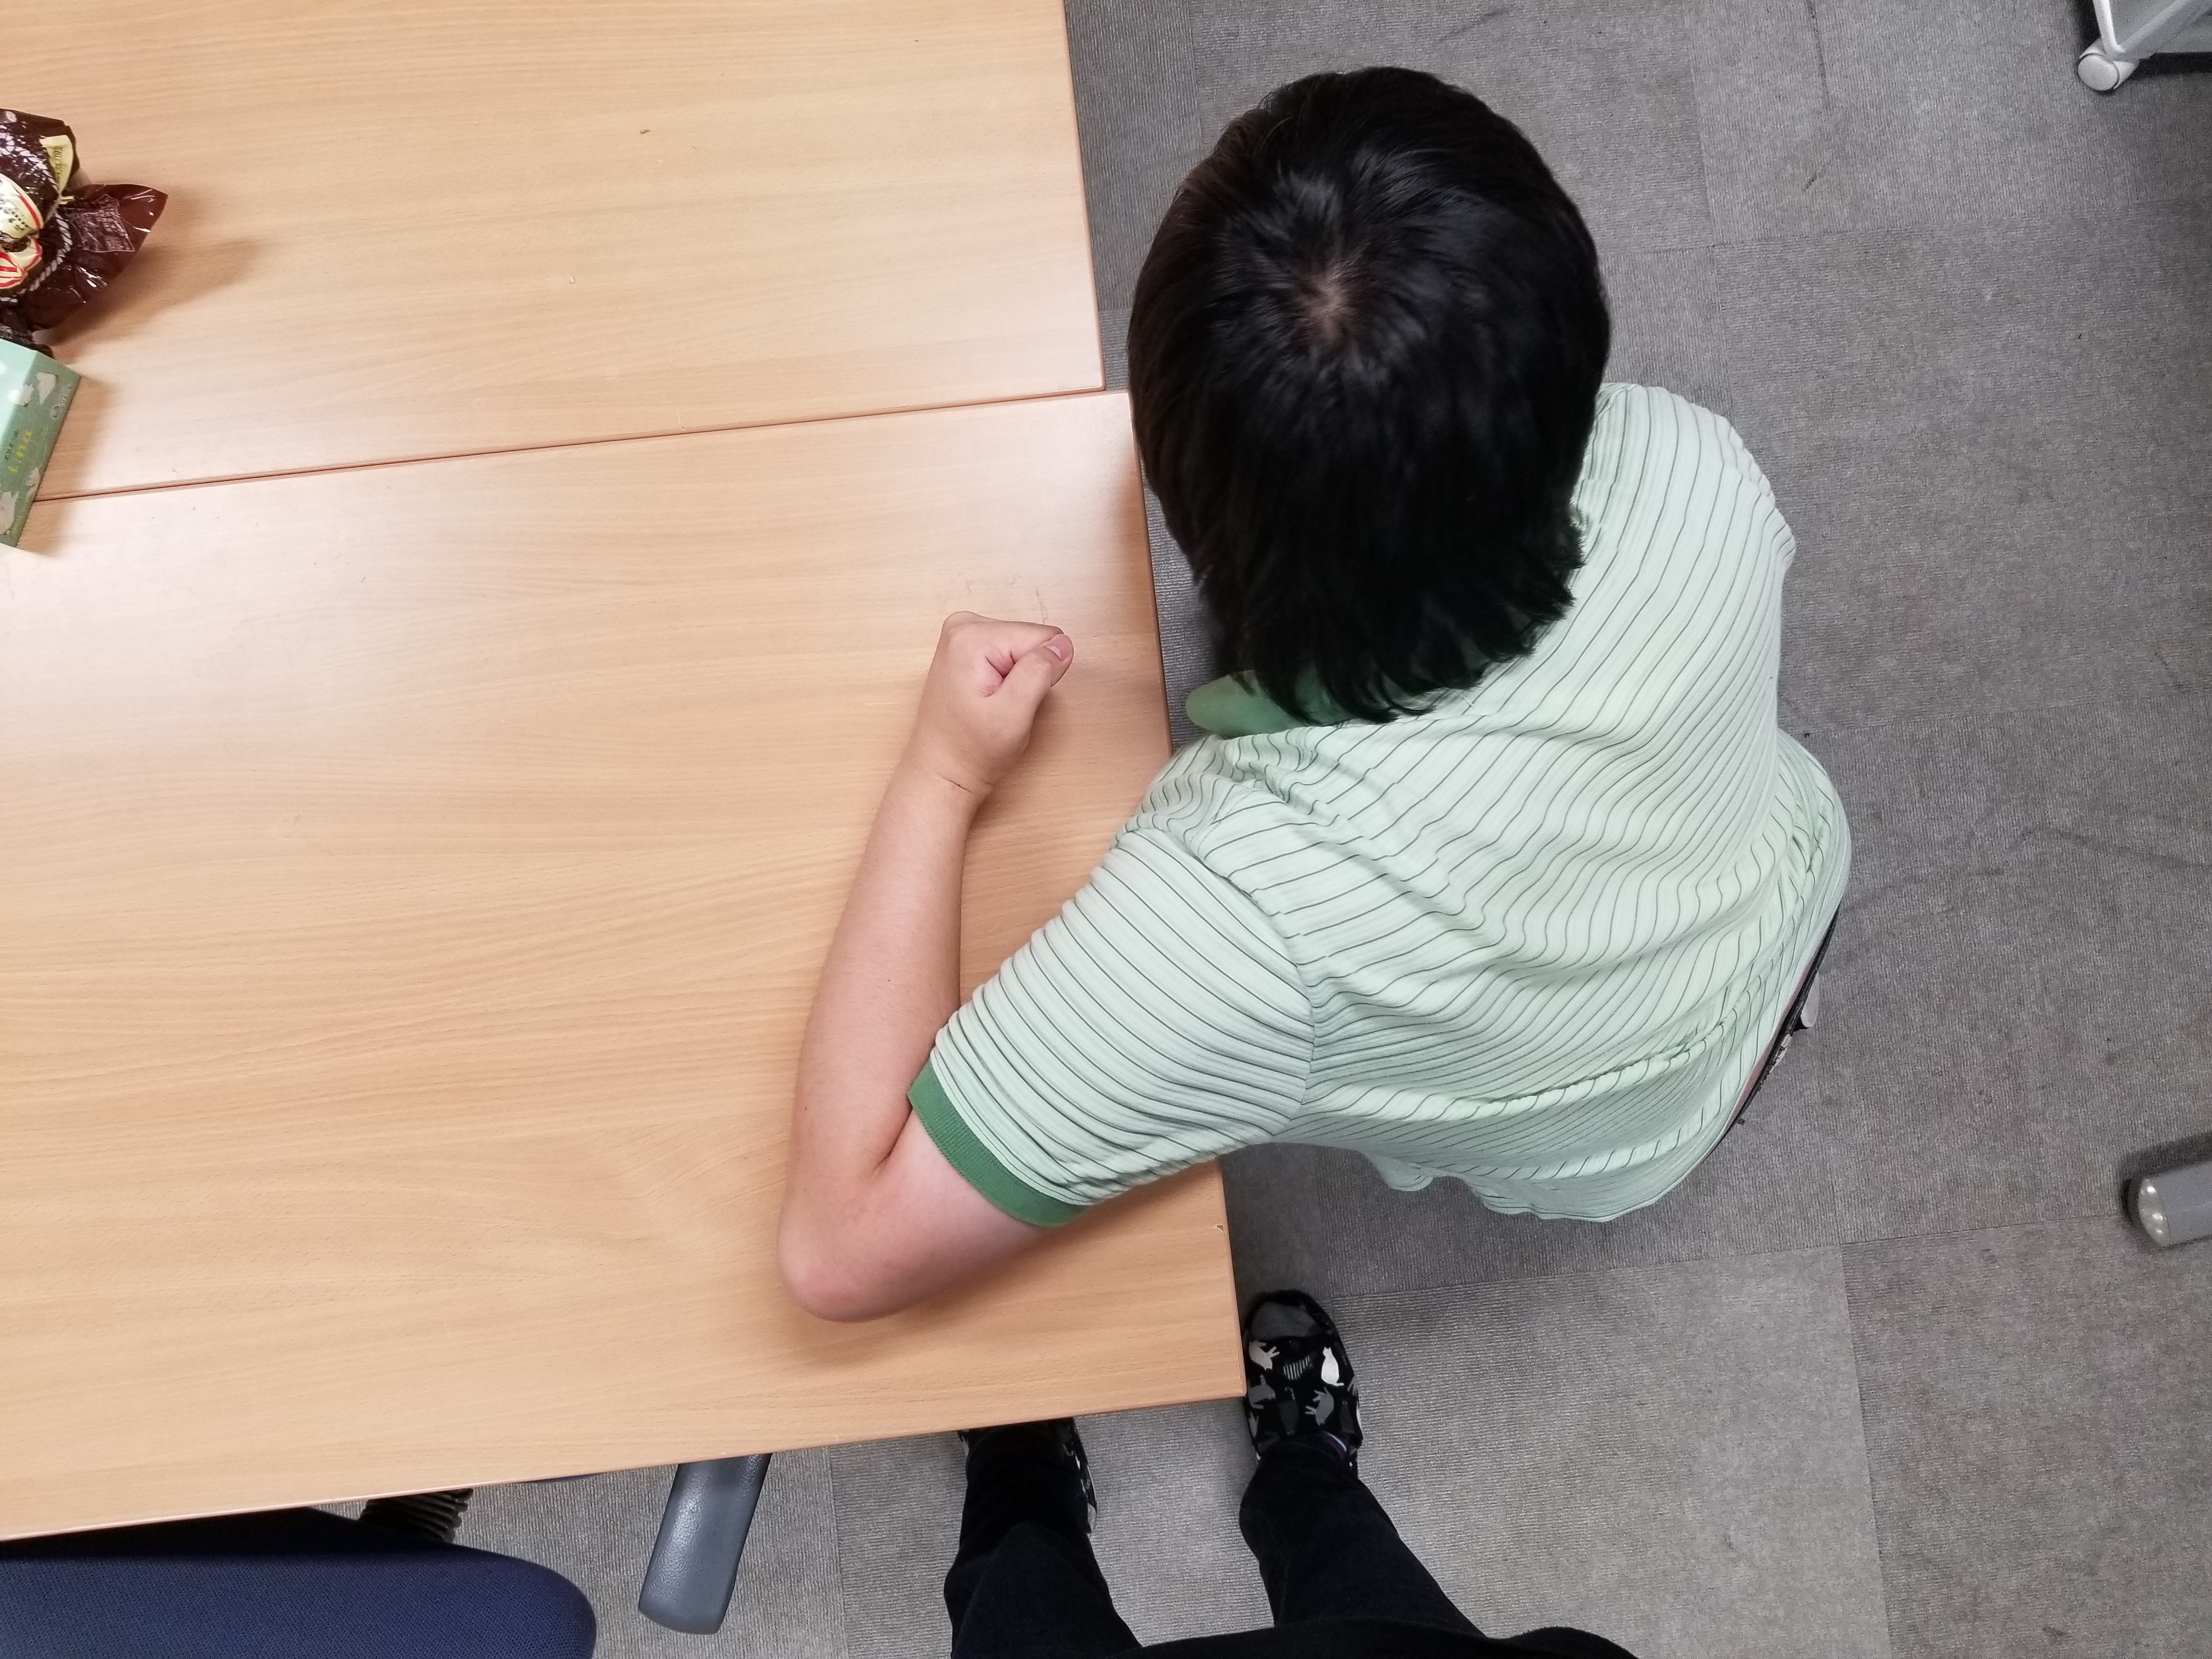
\includegraphics[width=7cm]{images/short.jpg}
\end{center}
\caption{腕を縮めた状態}
\label{fig:one}
\end{minipage}
\begin{minipage}{0.5\hsize}
\begin{center}
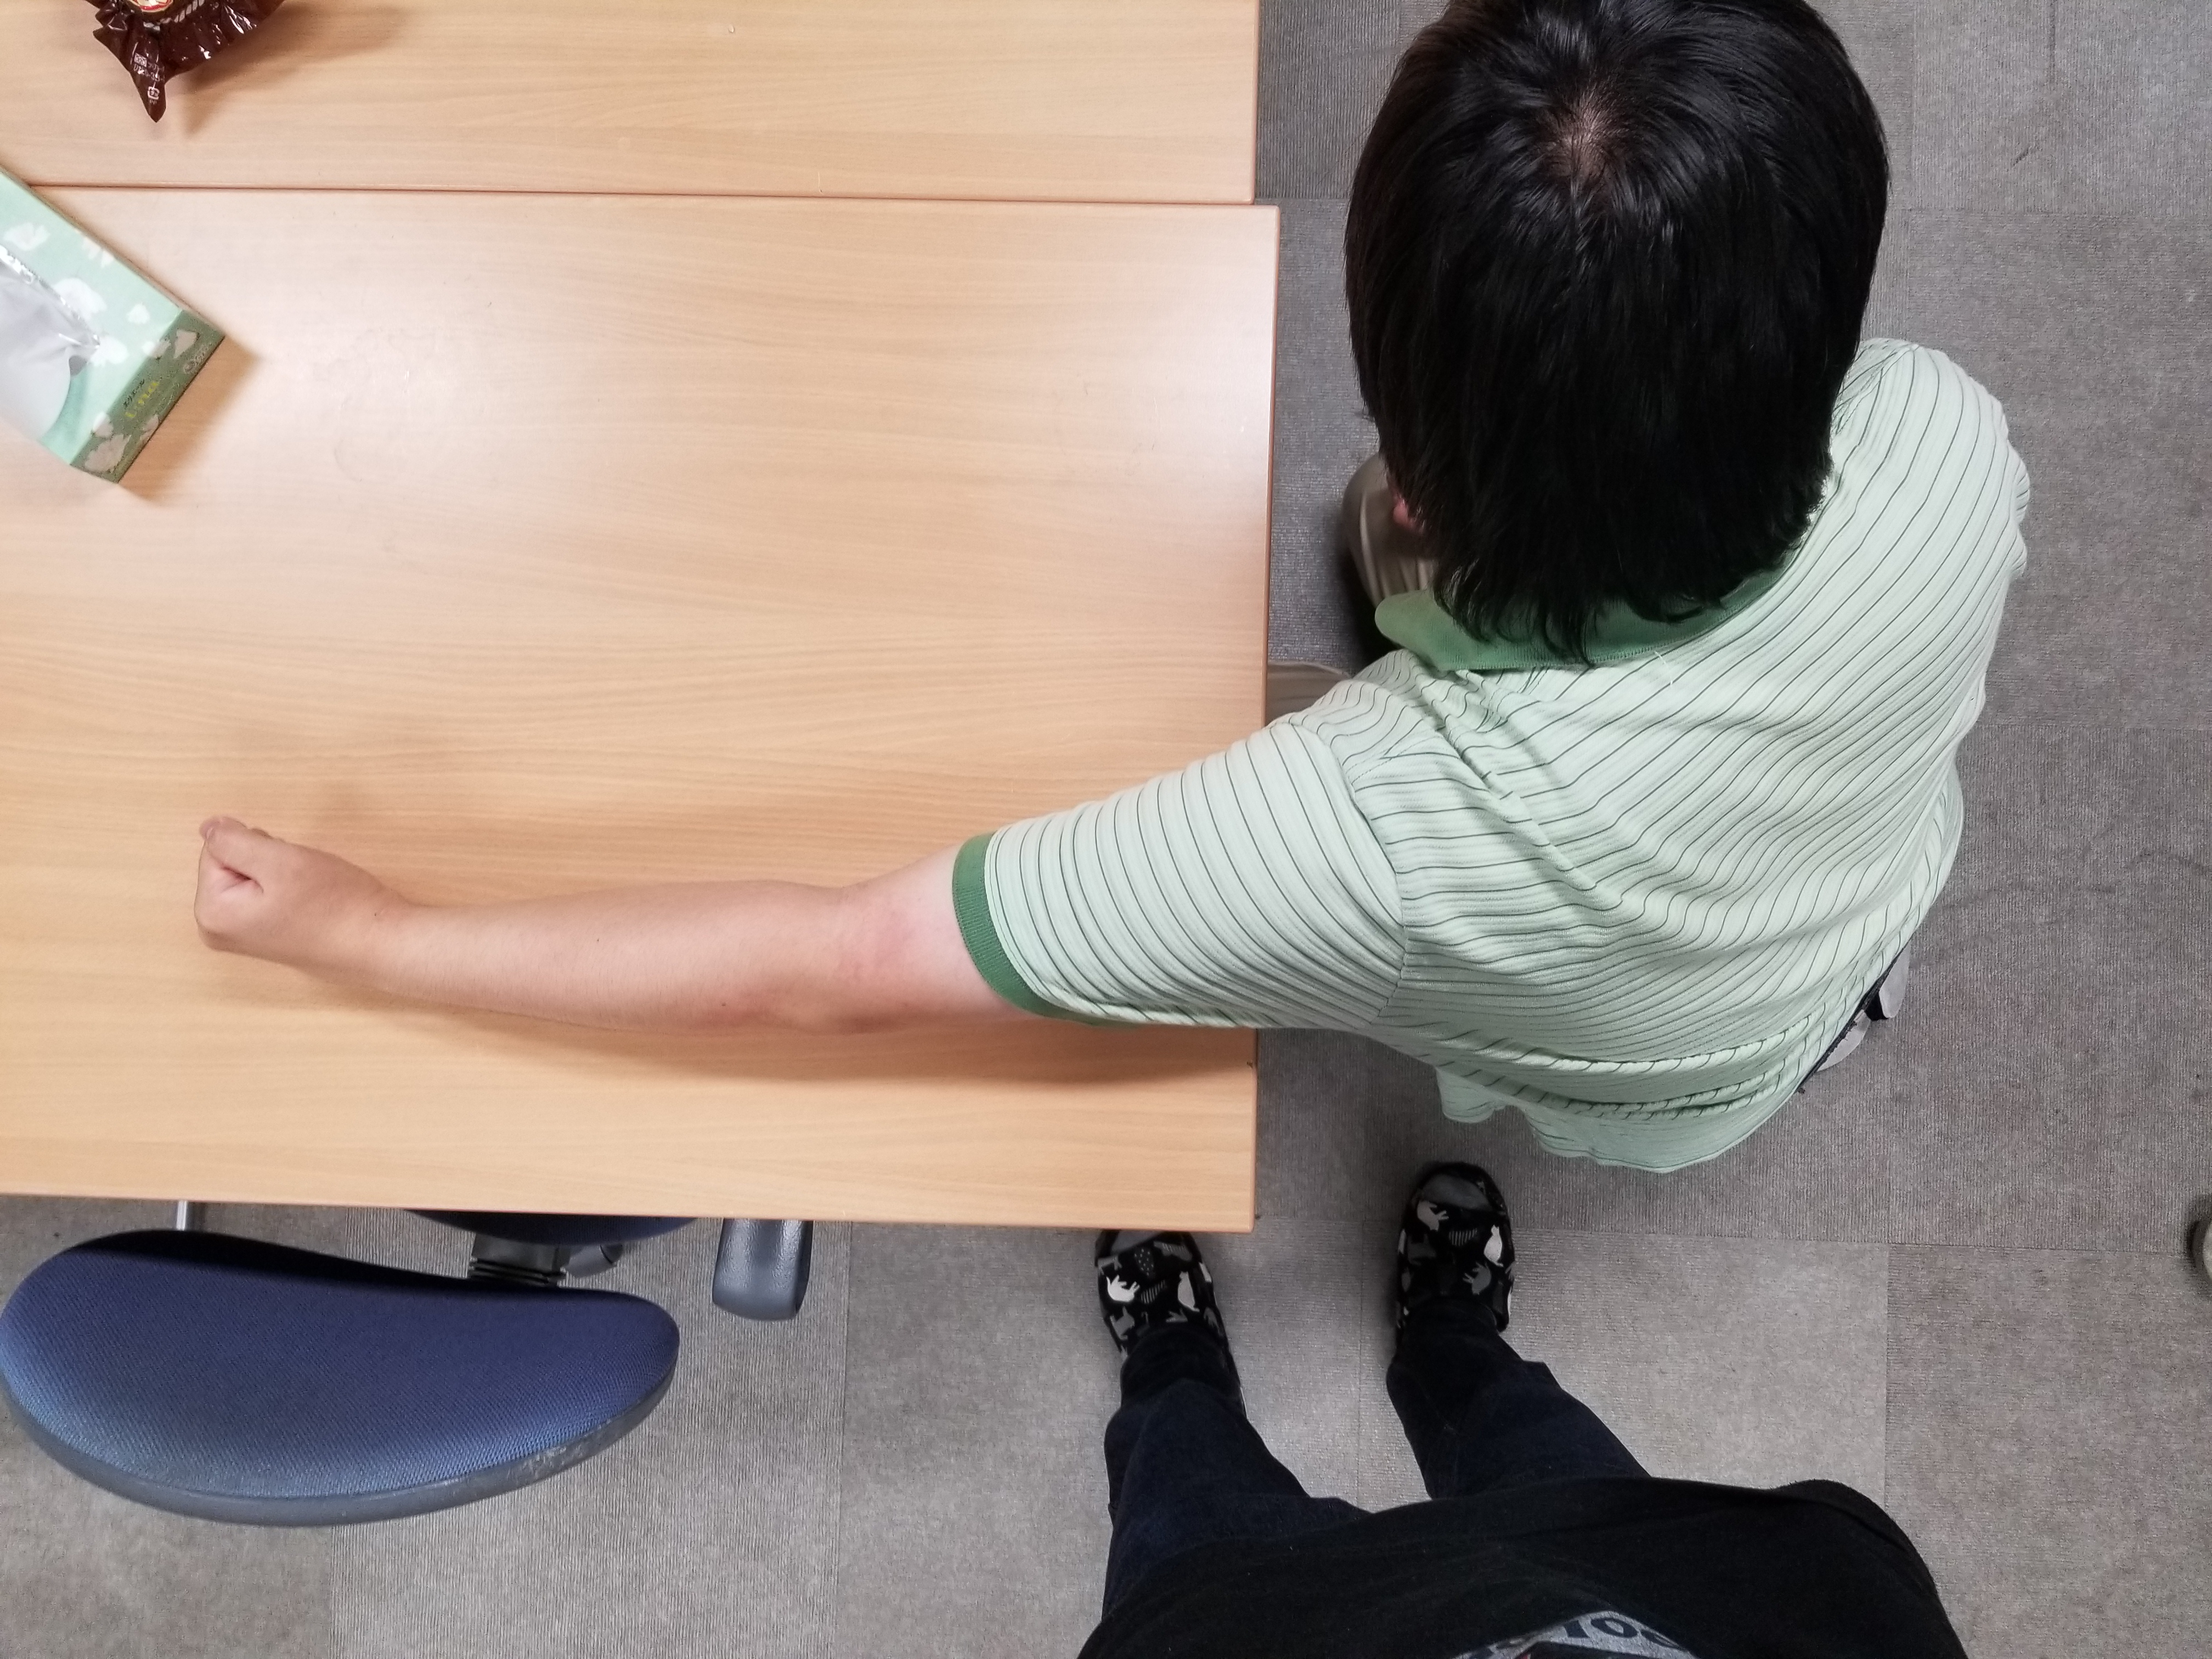
\includegraphics[width=7cm]{images/long.jpg}
\end{center}
\caption{腕を伸ばした状態}
\label{fig:two}
\end{minipage}
\end{figure}

計測した運動は、腕の曲げ伸ばし運動である。

上記の写真1と写真2を用いて具体的に説明すると、写真1の時をもっとも腕を曲げた状態、写真2の時を最も腕を伸ばした状態として、腕を伸ばしたり曲げたりという事を遅い速度と速い速度の2パターンで利き腕を使って被験者に行なってもらい、その様子を真上からカメラで撮影した。

\subsection{解析}
実験で計測した筋電計とモーションキャプチャーのデータをグラフにするための前処理を行った。

\subsubsection{筋電位}
筋電位のデータには以下の2つの処理を順番に施した。
\begin{description}
 \item[バンドパスフィルタ]\mbox{}\\
   データの中で、大きく外れるようなノイズを除去するために、通過帯域を1〜40Hzとしたバンドパスフィルタをかけた。しかし、バンドパスフィルタをかけることによってデータに位相ズレが生じるため、時間軸を反転してもう一度同じフィルタをかけることによってこれを補正した。
 \item[積分]\mbox{}\\
   このままでは筋肉の活動は電位の振れ幅でしか見ることができない。そこで積分を行い、面積として捉えることで筋肉の活動度を見る指標とした。積分式は以下のものを用いた。
   \begin{equation}
     a(t) = \frac{1}{\Delta T} \int_{t-\frac{\Delta T}{2}}^{t+\frac{\Delta T}{2}} |E(t)| dt
   \end{equation}
\end{description}

\subsubsection{位置座標}
体の位置座標のデータには3つの観測点、そしてそれぞれのx座標とy座標の位置データがある。さらにコマ数やフレーム間隔などの設定上のデータも付随しているため、データをグラフ化しやすくするためにデータの抜き出しをする必要があった。

具体的な処理では、
\begin{itemize}
 \item 位置座標のデータ部分と、設定などのそれ以外の部分に分ける。
 \item データ部から、位置情報を観測点ごとに分けて抜き出す。
\end{itemize}
というような処理を行った。
\newpage
\section{結果}
\begin{figure}[h]
\begin{center}
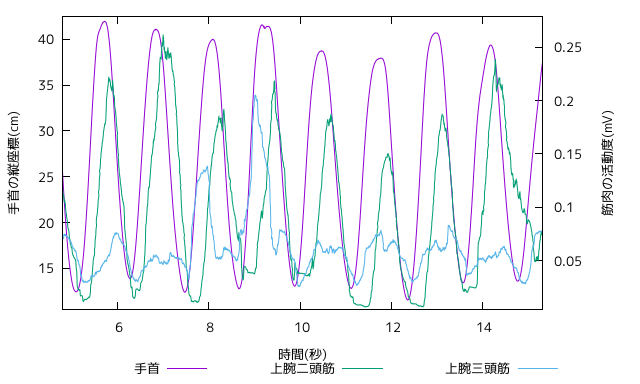
\includegraphics[width=16cm]{images/s1proto.png}
\end{center}
\caption{スロー時の運動と筋肉の活動度の関係}
\label{fig three}
\end{figure}
このグラフは、腕をゆっくり動かした時のものである。手首の縦軌道の座標を第一y軸に、筋肉の活動度を第二y軸に、そして時間をx軸とした。紫色のデータが手首の座標、緑色のデータが上腕二頭筋の筋肉活動度、青のデータが上腕三頭筋の筋肉活動度、である。観測点の中では手首の縦座標がもっとも移動が激しい部分のため、比較のために抜き出す部分とした。

このグラフからわかることは、上腕二頭筋は、ほとんどの場合で腕がもっとも曲げられた状態から、伸ばされ始めてから少しして活動度が大きくなっていっている。そして、腕を曲げるにしたがってその活動度を下げている。上腕三頭筋は、最大値が上腕二頭筋よりもかなり小さいが、同じような挙動をしている。しかし、いくつかの例においては、腕を伸ばし始めてから伸ばしきるまでの間だけ、上腕二頭筋に匹敵する活動度を見せているものもある。

\newpage
\begin{figure}[h]
\begin{center}
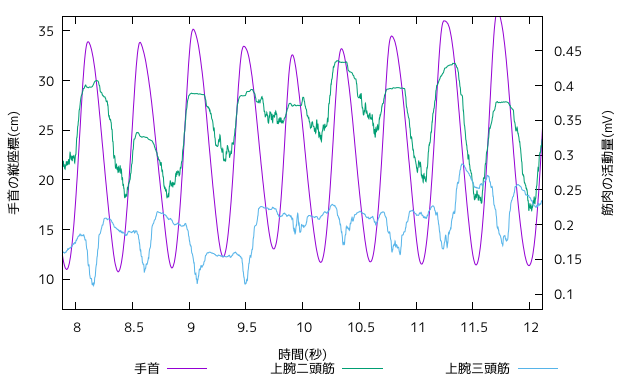
\includegraphics[width=16cm]{images/s2proto.png}
\end{center}
\caption{スロー時の運動と筋肉の活動度の関係}
\label{fig four }
\end{figure}
このグラフは、腕を速く動かした時のものである。軸や凡例は図3と同一のため、説明を省略する。

このグラフからわかることは、上腕二頭筋は、腕がもっとも曲げられた状態から、伸ばされ始めると同時に活動度が大きくなっていっている。そして、腕を曲げるにしたがってその活動度を下げている。上腕三頭筋は、腕を伸ばしきった状態で縮曲げ始め、再び腕を伸ばしきる直前まで大きな活動度を示している。
\section{考察}
私は、上腕二頭筋は腕を縮めるときに、上腕三頭筋は腕を伸ばすときだけに使うものと考えていた。しかし、上腕二頭筋は腕を
伸ばすときにも、上腕三頭筋は腕を曲げるときにも、それぞれ使われていることが計測で分かった。

人は、片側の筋肉だけでは動作の速度をうまく調整できずに想定した速さより速くなってしまう。そこで、反対側の筋肉(二頭筋なら三頭筋。三頭筋なら二頭筋)を使うことによって移動方向と逆側に力を加えて速さを調整しているのではないか、と私は考える。

そうすれば、伸ばすときに上腕二頭筋を、曲げるときに上腕三頭筋を使っていることの説明ができるだろう。
\end{document}

